\documentclass[uplatex]{jsarticle}
\usepackage[dvipdfmx]{graphicx}
\title{ソフトウェア設計法3}

\author{101730153 佐治 礼仁 saji.ayahito@h.mbox.nagoya-u.ac.jp}
\date{\today}
\begin{document}
\maketitle
\section{電車の自動改札をICカードで出場する場合の、ユースケース図、クラス図、シーケンス図を書け。}
\subsection{ユースケース図}
ユースケース図を図\ref{fig:usecase-diagram}に記載する.
\begin{figure}[htbp]
  \begin{center}
    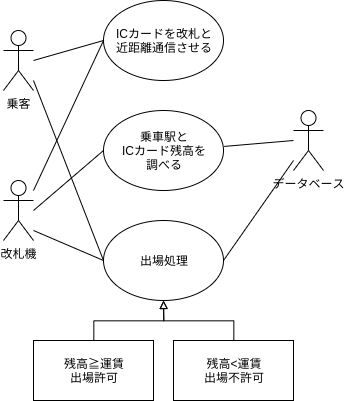
\includegraphics[clip,width=7.5cm]{figures/usecase-d.png}
    \caption{ユースケース図}
    \label{fig:usecase-diagram}
  \end{center}
\end{figure}
\subsection{クラス図}
クラス図を図\ref{fig:class-diagram}に記載する.
\begin{figure}[htbp]
  \begin{center}
    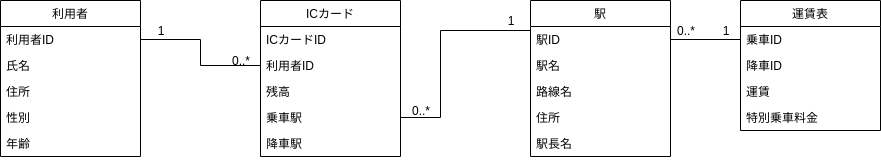
\includegraphics[clip,width=12.0cm]{figures/class-d.png}
    \caption{クラス図}
    \label{fig:class-diagram}
  \end{center}
\end{figure}
\subsection{シーケンス図}
シーケンス図を図\ref{fig:sequence-diagram}に記載する.
\begin{figure}[htbp]
  \begin{center}
    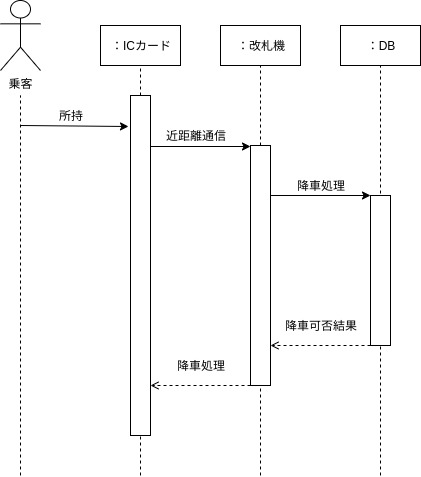
\includegraphics[clip,width=7.5cm]{figures/sequence-d.png}
    \caption{シーケンス図}
    \label{fig:sequence-diagram}
  \end{center}
\end{figure}
\end{document}
